\documentclass[a4paper,titlepage]{article}
\usepackage[utf8]{inputenc}
\usepackage[ngerman]{babel}
\usepackage[T1]{fontenc}
\usepackage{geometry}
\usepackage{times}
\geometry{a4paper,left=40mm,right=20mm,top=2cm,bottom=2cm}
\usepackage{graphicx}
\usepackage{amsmath,amsfonts,amssymb}
\usepackage{multirow}
\numberwithin{equation}{section} %Nummeriert mathematische Umgebungen nach sections durch
\usepackage[nodisplayskipstretch]{setspace} %lässt Abstand zwischen align-Umgebungen und Text auf 1.0
\setstretch{1.5}% ergibt 1,5-fachen Zeilenabstand
%%%%%%%%%%%%%%%%%%%%%%%%%%%%%%%%%%%%%%%%%%%%%%%%%%%%%%%%%%%%%%%%%%%%%%%%%%%%%%%%%%%%%%%%%%%%%%%%


%%%%%%%%%%%%%%%%%%%%%%%%%%%%%%%%%%%%%%%%%%%%%%%%%%%%%%%%%%%%%%%%%%%%%%%%%%%%%%%%%%%%%%%%%%%%%%%%

\begin{document}
\begin{titlepage}
\begin{center}                     
        {\Large\scshape \textbf{Project ML}}\\*[2mm]
				{\large University of Hamburg}\\*[0mm]

				{\large Department of Mathematics}\\*[0mm]
				{\large \emph{Jonas Eckhoff - Timo Greve\\ 
Max Lewerenz - Giulia Satiko Maesaka - John-Robert Wrage}}\\*[30mm]
				

        {\bf \LARGE Machine Learning Methods
         \\ Group 5}\\*[12mm]

\end{center}  

\end{titlepage}
\newpage

%%%%%%%%%%%%%%%%%%%%%%%%%%%%%%%%%%%%%%%%%%%%%%%%%%%%%%%%%
%%%%%%%%%%%%%%%%%%%%%%%%%%%%%%%%%%%%%%%%%%%%%%%%%%%%%%%%%

\pagenumbering{Roman}
\setcounter{page}{2}

\tableofcontents
\newpage

\addcontentsline{toc}{section}{List of figures}
\listoffigures
\newpage

%\addcontentsline{toc}{section}{Tabellenverzeichnis}
%\listoftables
\newpage

%%%%%%%%%%%%%%%%%%%%%%%%%%%%%%%%%%%%%%%%%%%%%%%%%%%%%%%%%
%%%%%%%%%%%%%%%%%%%%%%%%%%%%%%%%%%%%%%%%%%%%%%%%%%%%%%%%%

\pagenumbering{arabic}
\setcounter{page}{1}
\section{Introduction}

What is this paper for?
What are the main goals?

E.g.
this is for ourself. We want to build an overview about the common algorithms, how they work and their advantages/disadvatages.

\newpage

%%%%%%%%%%%%%%%%%%%%%%%%%%%%%%%%%%%%%%%%%%%%%%%%%%%%%%%%%
%%%%%%%%%%%%%%%%%%%%%%%%%%%%%%%%%%%%%%%%%%%%%%%%%%%%%%%%%


\section{What is ML?}
First some words about ML. Maybe from Lotz, first chapter?
Next we could use this grapic to visualize the topic.
\begin{figure}[hbtp]
	\centering
	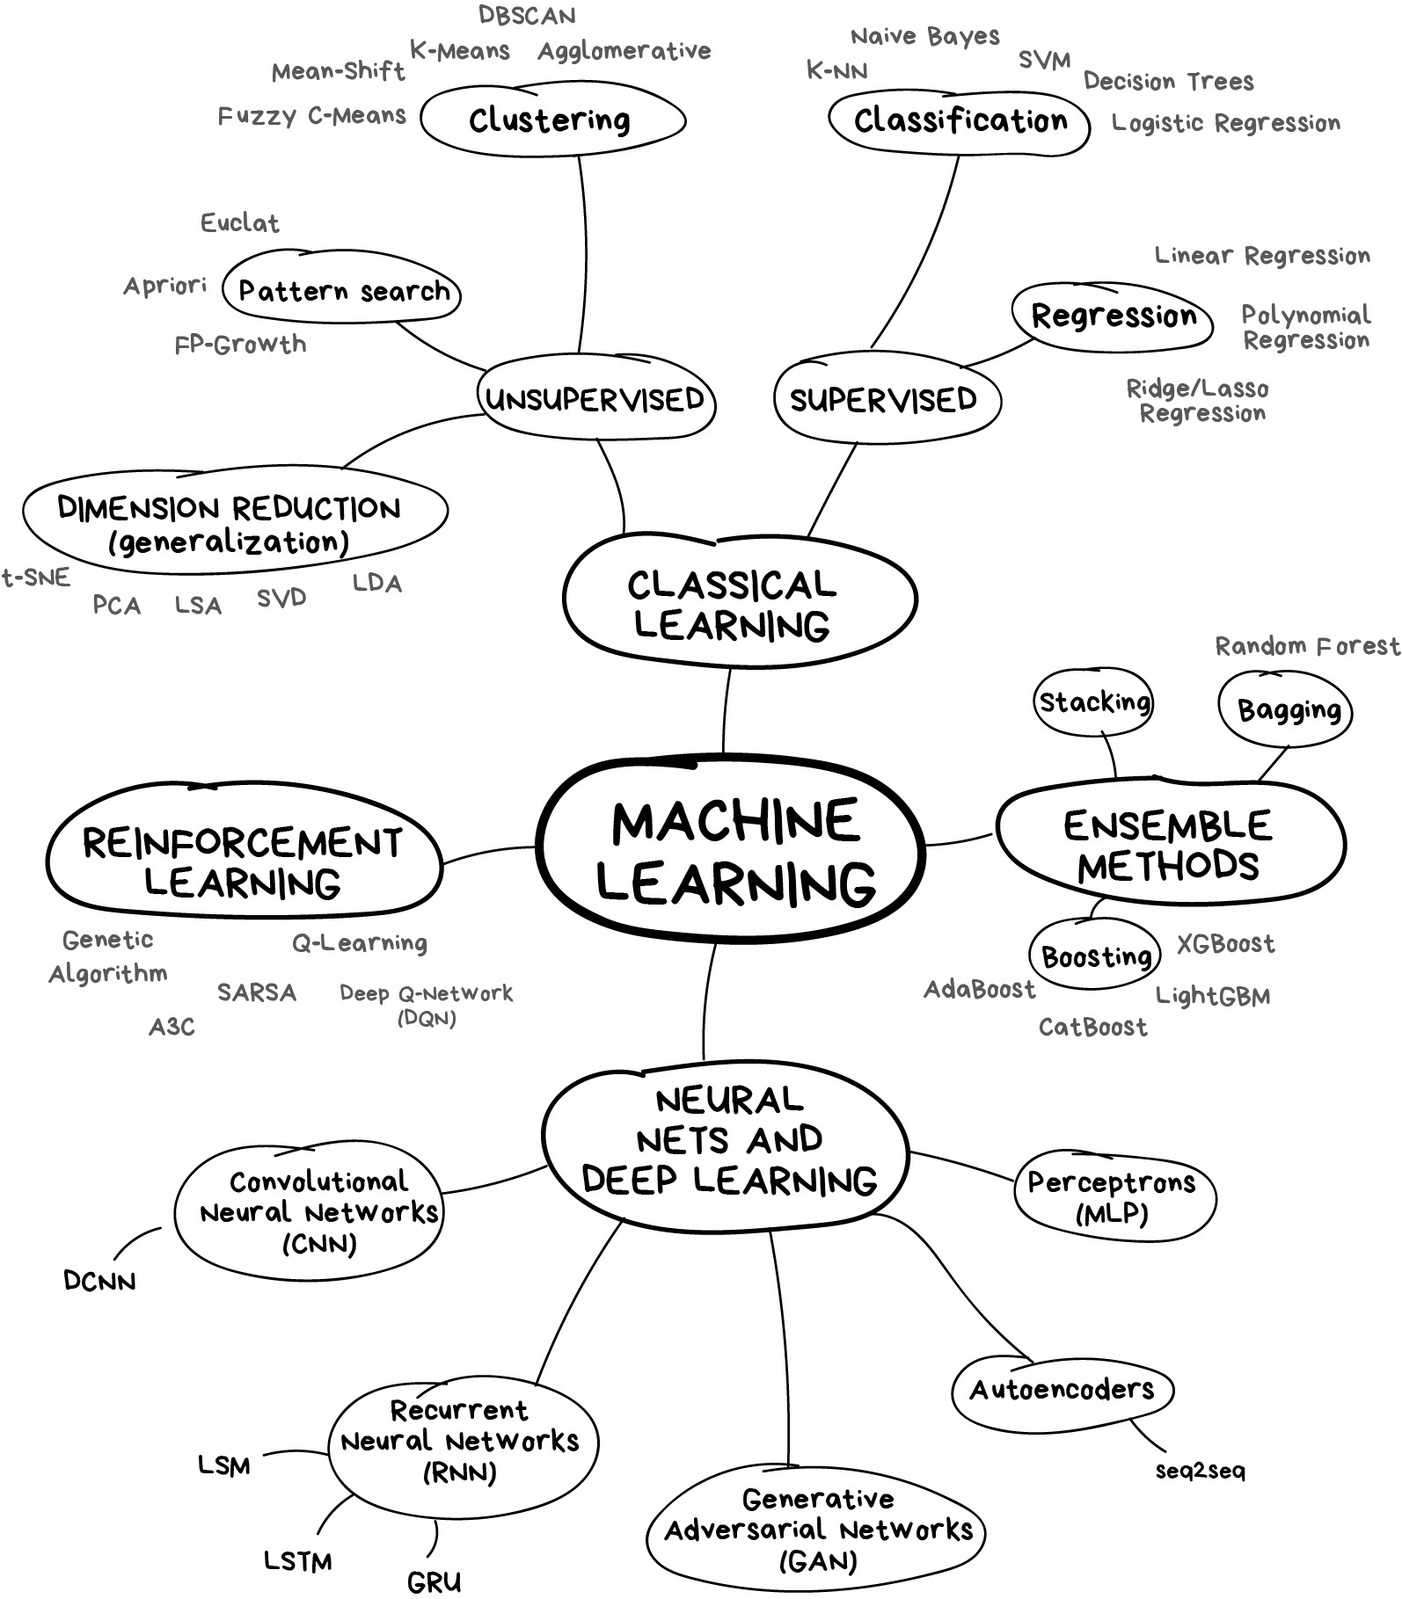
\includegraphics[width=1\textwidth]{ML}
	\caption{ML-Overview}
	% \vspace{-20pt}
	\label{fig:Datensatz - unbearbeitet}
\end{figure}

Finally i would sugest to finish with a Table.

I would structure it like:
Algorithm, Main Idea(in like 3-5 sentences), possible application(image processing, clustering, etc.) advantages, disadvantages

%%%%%%%%%%%%%%%%%%%%%%%%%%%%%%%%%%%%%%%%%%%%%%%%%%%%%%%%%

\subsection{Basis ML 1(maybe Data)}
We could speak a lil bit more about data in this topic?




%%%%%%%%%%%%%%%%%%%%%%%%%%%%%%%%%%%%%%%%%%%%%%%%%%%%%%%%%

\subsection{Basis ML 2}
TBA





\newpage
%%%%%%%%%%%%%%%%%%%%%%%%%%%%%%%%%%%%%%%%%%%%%%%%%%%%%%%%%
%%%%%%%%%%%%%%%%%%%%%%%%%%%%%%%%%%%%%%%%%%%%%%%%%%%%%%%%%

\section{Classical learning}
Difference between Supervised unsupervised.


%%%%%%%%%%%%%%%%%%%%%%%%%%%%%%%%%%%%%%%%%%%%%%%%%%%%%%%%%

\subsection{Supervised}
Um einen Abfragepunkt zu klassifizieren, nutzt diese Methode die gespeicherten

%%%%%%%%%%%%%%%%%%%%%%%%%%%%%%%%%%%%%%%%%%%%%%%%%%%%%%%%%

\subsubsection{Regression}
Like for all other subsubsections i would sugest that we structure the Algorithms like in the table at Ch.2.(\textbf{\underline{Algorithm}}, \textbf{\underline{possible application}}, etc.), but also add some links etc. Trainingsdaten und berechnet den Abstand zu den jeweiligen Merkmalen. In 
 
%%%%%%%%%%%%%%%%%%%%%%%%%%%%%%%%%%%%%%%%%%%%%%%%%%%%%%%%%

\subsubsection{Classification}
See regression
%%%%%%%%%%%%%%%%%%%%%%%%%%%%%%%%%%%%%%%%%%%%%%%%%%%%%%%%%

\subsection{Unsupervised}
See regression

%%%%%%%%%%%%%%%%%%%%%%%%%%%%%%%%%%%%%%%%%%%%%%%%%%%%%%%%%

\subsubsection{Clustering}
See regression
 
%%%%%%%%%%%%%%%%%%%%%%%%%%%%%%%%%%%%%%%%%%%%%%%%%%%%%%%%%

\subsubsection{Pattern search}
See regression
%%%%%%%%%%%%%%%%%%%%%%%%%%%%%%%%%%%%%%%%%%%%%%%%%%%%%%%%%

\subsubsection{Dimension Reduction}
See regression

%%%%%%%%%%%%%%%%%%%%%%%%%%%%%%%%%%%%%%%%%%%%%%%%%%%%%%%%%
 


\newpage

%%%%%%%%%%%%%%%%%%%%%%%%%%%%%%%%%%%%%%%%%%%%%%%%%%%%%%%%%
%%%%%%%%%%%%%%%%%%%%%%%%%%%%%%%%%%%%%%%%%%%%%%%%%%%%%%%%%

\section{Neural nets and deep learning}
Maybe we can use the insights we generate while solving our problem to fill this chapter.


%%%%%%%%%%%%%%%%%%%%%%%%%%%%%%%%%%%%%%%%%%%%%%%%%%%%%%%%%

\subsection{Convolutional Neural Networks CNN}


%%%%%%%%%%%%%%%%%%%%%%%%%%%%%%%%%%%%%%%%%%%%%%%%%%%%%%%%%

\subsection{Recurrent Neural Networks RNN}

%%%%%%%%%%%%%%%%%%%%%%%%%%%%%%%%%%%%%%%%%%%%%%%%%%%%%%%%%

\subsection{Generative adversarial networks GAN}

%%%%%%%%%%%%%%%%%%%%%%%%%%%%%%%%%%%%%%%%%%%%%%%%%%%%%%%%%

\subsection{Autoencoders}


%%%%%%%%%%%%%%%%%%%%%%%%%%%%%%%%%%%%%%%%%%%%%%%%%%%%%%%%%

\subsection{Perceptrons MLP}


%%%%%%%%%%%%%%%%%%%%%%%%%%%%%%%%%%%%%%%%%%%%%%%%%%%%%%%%%


\newpage


%%%%%%%%%%%%%%%%%%%%%%%%%%%%%%%%%%%%%%%%%%%%%%%%%%%%%%%%%
%%%%%%%%%%%%%%%%%%%%%%%%%%%%%%%%%%%%%%%%%%%%%%%%%%%%%%%%%

\section{Ensemble Methods}



%%%%%%%%%%%%%%%%%%%%%%%%%%%%%%%%%%%%%%%%%%%%%%%%%%%%%%%%%

\subsection{Bagging}


%%%%%%%%%%%%%%%%%%%%%%%%%%%%%%%%%%%%%%%%%%%%%%%%%%%%%%%%%

\subsection{Boosting}


%%%%%%%%%%%%%%%%%%%%%%%%%%%%%%%%%%%%%%%%%%%%%%%%%%%%%%%%%

\subsection{Stacking}


\newpage

%%%%%%%%%%%%%%%%%%%%%%%%%%%%%%%%%%%%%%%%%%%%%%%%%%%%%%%%%
%%%%%%%%%%%%%%%%%%%%%%%%%%%%%%%%%%%%%%%%%%%%%%%%%%%%%%%%%

\section{Reinforcement learning}


\newpage

%%%%%%%%%%%%%%%%%%%%%%%%%%%%%%%%%%%%%%%%%%%%%%%%%%%%%%%%%
%%%%%%%%%%%%%%%%%%%%%%%%%%%%%%%%%%%%%%%%%%%%%%%%%%%%%%%%%

\begingroup
\addcontentsline{toc}{section}{Bibliography}
\renewcommand*\refname{Bibliography}

\begin{thebibliography}{----}
% Check - Korrekt 

\bibitem{Deutsche Aktuarvereinigung e.V.}
\textsc{Deutsche Aktuarvereinigung e.V.}, 2012: Unisex-Tarifierung, abgerufen am 10. November 2019: https://aktuar.de/fachartikelaktuaraktuell/Lebensversicherung{\_}Unisex{\_}Aktuar-aktuell{\_}19.pdf{\#}search=unisex

\bibitem{Ertel2016}
\textsc{Ertel}, W. (2016): {\it Grundkurs Künstliche Intelligenz}. Springer Vieweg, Wiesbaden. 4. Auflage.


\end{thebibliography}
\endgroup


\newpage



\end{document}
